\section{One-PE Platform}
\label{sec:onehost}

With a single PE, only one task can execute at a time and rollback/recovery is the only way to cope with failures.  For a single task, with fixed execution time and zero restart overhead, computing the probability of completion by a deadline is non-trivial as it requires characterizing the ``longest gap" distribution of a Poisson process~\cite{OMWONYLEE2020124194}.  Furthermore, when considering a chain of tasks there is a continuum of possible values for the time remaining until the deadline at the next scheduling decision.  To make the continuous-time scheduling problem tractable, we thus discretize time. 
For a given application, we use dynamic programming to precompute scheduling decisions in time polynomial in the number of discrete time intervals, and $O(1)$-time scheduling decisions at runtime.


\subsection{Scheduling Strategy}
\label{sec:onehost:solution}

Let time be discretized as a sequence of time steps 
of duration \deltat, so that all time durations are
integral numbers of time steps. The execution time for 
execution mode $j$ of task $T_i$, for $x$ bytes of input data 
with error level $y$ is then: 
$$
m^i_j = \left\lceil \frac{x/B_r + t^i_j(x,y) + d^i_j(x,y)/B_w}{\deltat} \right\rceil ,
%m^i_j = \left\lceil (x/B_r + t^i_j(x,y) + d^i_j(x,y)/B_w) / \deltat \right\rceil ,
$$
\noindent
where the numerator is the time to read the input, to perform
the computation, and to write the output. 

Let us consider an execution that conforms to a ``first-output" policy
by which a task is never re-executed once it has completed
successfully once.  This implies that the application execution stops as
soon as one execution of task $T_M$ has succeeded. Imposing this
restriction makes the recursion hereafter more tractable and, more
importantly, limits the state space size of the corresponding dynamic program.

We define $E(i, x, y, n)$ as the optimal expected error (with discretized time)
when executing $T_{i}$ to
$T_{M}$ for $i{=}1,\ldots,M$, where the input to $T_{i}$ is $x$ bytes
with error level $y$, given that there are $n$ time steps until the
deadline.  If $\forall j\; m_j^i{>}n$, then $E(i, x, y, n){=}\efail$, since
there is no possibility of completing $T_{i}$ by the deadline.
Otherwise, recursively:
\begin{multline}
\label{eq:dp1}
E(i, x, y, n) = 
    \min_{1\leq j \leq K_i,\; s.t.\; m_j^i \leq n} \big[\\
\psuc{m_{j}^i} \times E(i+1, d_j^i(x,y), e_j^i(x,y), n - m_j^i) + \\
	\sum_{u=0}^{m_j^i - 1} p_u E(i, x, y, \max(0, n - u - 1 - \lceil R/\deltat \rceil)) \big],
\end{multline}
\noindent
where $p_u{=}\psuc{u}{-}\psuc{(u+1)}$, i.e., the probability that a failure
occurs during time step $u$, where time step 0 is the first time step. 
The above expression is the minimum expected error over all feasible execution modes used for the upcoming execution of $T_{i}$.  The first term 
is for the case in which there is no failure during the execution of $T_{i}$ with execution mode $j$, which happens with probability
$\psuc{m_{j}^i}$. In this case, the execution will proceed with
$T_{i+1}$, with input data size and error level based on the
output from $T_{i}$, and with 
$m_j^i$ fewer time steps remaining until the deadline. The second term considers all time steps at which the
execution of $T_{i}$ can fail. Failing during time step $u$ happens with
probability $p_u$ and will cause a re-execution of $T_i$ but with
$u{+}1{+}\lceil R/\deltat \rceil$ fewer
time steps until the deadline.  The base case is
simply $E(M+1, x, y, n) = y\;$.

%$E(M, x, y, n)$, is when only $T_{M}$ is left to execute. 
%$E(M, x, y, n)$ is equal to $\efail$ if $\forall j\; m_j^M{>}n$  (i.e., there are no feasible execution modes). Otherwise, recursively:
%\begin{multline}
%E(M, x, y, n) = \min_{1\leq j \leq K_M,\; s.t.\; m_j^M \leq n} \big[\psuc{m_{j}^M} \times e_j^M(x,y)\\
%	+ \sum_{u=0}^{m_j^M - 1} p_u E(M, x, y, \max(0, n - u - 1 - \lceil R/\deltat \rceil)) \big].
%\end{multline}
%The only difference with Equation~\eqref{eq:dp1} is that if $T_M$ succeeds
%with execution mode $j$, then the recursion ends and the output error
%s simply $e_j^M(x,y)$.

The above recursion provides a dynamic programming solution for
precomputing all scheduling decisions.  The initial decision is to select
an execution mode that attains the minimum in the expression for $E(1,x_0, y_0,
H)$, where $x_0$ and $y_0$ are the size and error of the input to task
$T_1$, and $H{=}\lfloor D/\deltat \rfloor$.  Note that the number of time
steps until the deadline is rounded downward, while we round task execution
times and restart overheads upward, so that an execution computed in
discretized time is guaranteed to be feasible in continuous time.  Using
memoization, all reachable values $E(i, x, y, n)$, together with the
execution modes attaining their minima, can be precomputed and stored in a
table.  At runtime, whenever the PE is idle, the execution mode for the
current state $(i, x, y, n)$ can be selected in $O(1)$ time by looking up
the table.

Let us denote by $Q$ the number of possible size/error pairs for the input
provided to all tasks, and let $K{=}\max_i K_i$. The time complexity for
the above algorithm is $O(KQH^2)$, and the size of the computed table is
$O(QH)$. The table could be compressed by storing, for each state $(i,x,y)$,
maximal intervals of values for which
the selected mode is unchanged.  Regardless, for a fixed application
specification, the time and space complexities are pseudo-polynomial in
the numerical deadline.  Although $Q$ may be exponential in the number of
tasks, the algorithm remains practical (see results in the next section).
Besides, for a given application and failure rate, the algorithm is
invoked offline only once, and the computed table can be reused for all
executions of the application.



%\HC{This following paragraph could be removed or heavily modified based on the TODOs hereafter}
%When the application consists of a single task, one can prove that the set
%of time steps until the deadline can be partitioned into time intervals,
%and that one can compute in pseudo-polynomial time the optimal execution
%mode to use when a decision is made at any point in each of these
%intervals.  In this manner, one can precompute a table of size $O(K_1)$,
%and at runtime one can select the optimal execution mode to use for the
%next task execution with complexity $O(\log K_1)$ using binary search.
%This result, however, does not seem to generalize to chains of more than
%one task. We thus omit it here due to lack of space.

Recall that the above approach is for a first-output policy. Due to the randomness of
failures the application may complete well ahead of the deadline.  A
natural idea is then to use opportunistic \emph{temporal redundancy} and
attempt subsequent application executions. Integration of this idea in our
recursion would require an enlarged state space.  Instead, we perform
temporal redundancy as a separate re-execution step after $T_M$ completes.
Each such re-execution is computed while excluding task mode sequences
that cannot possibly improve on the error level achieved by the previously
completed execution. It is straightforward to remove these execution modes
from consideration and, provided any viable execution modes remain, apply
our scheduling strategy again. The extent to which this temporal redundancy
technique is useful depends on the application specification, the failure
rate, the restart overhead, and the deadline. In our experimental results,
when using this technique, we always restart the application
from task $T_1$.  Assuming that
intermediate task output data from the previous execution are still
available in stable storage, the re-attempted execution could start
with task $T_{i_0}$, $i_0 > 1$. We leave investigating this possibility, including
the problem of determining the best $i_0$, for future work.


\subsection{Discretization Selection}

A practical question is: what value of $\deltat$ should be used?  A
smaller $\deltat$ value yields a better approximation of the continuous-time problem,
but leads to higher complexity due to a larger number of time steps.  
Although the algorithm needs to be invoked only once, a user could still wish
to determine the largest value of $\deltat$ that leads to accuracy within
some tolerance.

The developments in the previous section actually compute a pessimistic
upper bound on the optimal continuous-time expected error for the first-output
policy.  This is because the dynamic program is invoked for the deadline
rounded downward, all task durations $m^i_j$ are rounded upward, the
restart overhead is rounded upward, and a failure at any point in a time
interval ``wastes" that entire interval.  Small modifications make it
possible to compute an optimistic lower bound: invoke the
dynamic program for the deadline rounded upward; round all $m^i_j$ task
durations downward; and replace $n{-}u{-}1{-}\lceil R/\deltat\rceil$ by
$n{-}u{-}\lfloor R/\deltat \rfloor$ in the recursive expressions.  Note
that for $u=0$, if $\lfloor R / \deltat \rfloor = 0$ there is a self-loop in
the recursion. In this case we disregard the $u=0$ term in the summation
(and renormalize probabilities).

\begin{figure}[ht!]
	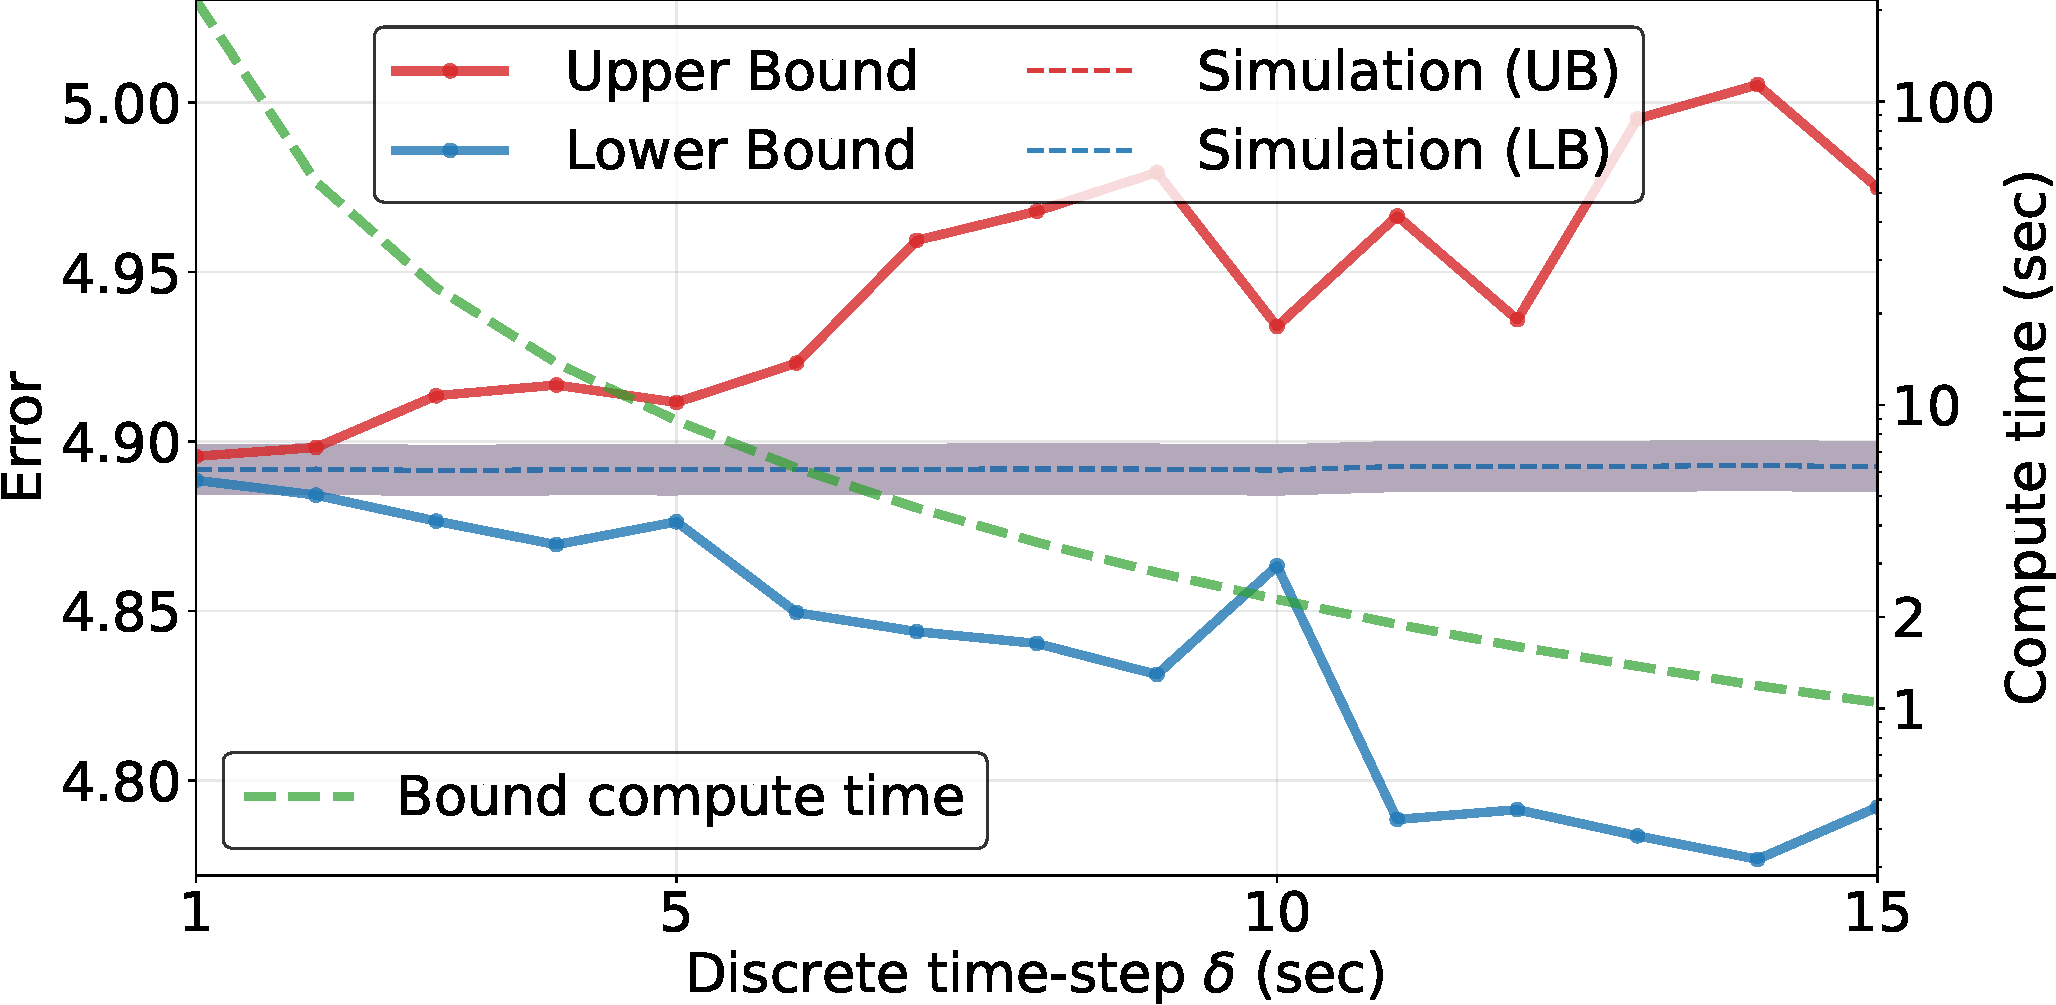
\includegraphics[width=\columnwidth]{./figures/delta_t_results.pdf}	
	\caption{Expected error bounds, sample simulated
	error for 5 million repeats (95\% confidence interval shown by
	shaded region), and bound computation time vs. $\deltat$, for the
	fusion science use case in Section~\ref{sec:use-case}.}
	\label{fig:delta_t}

\end{figure}

In practice, a user would pick a value for \deltat so that the difference
between the two bounds is below some threshold, and then make scheduling
decisions according to the dynamic program for the lower bound or for the
upper bound. For instance, Fig.~\ref{fig:delta_t} plots the two bounds
vs. \deltat for the use case in Section~\ref{sec:use-case}.  As expected,
the distance between the two bounds increases as \deltat increases. But
the increase is not monotonic, as seen in the jagged shape of the
curves. This behavior is easily explained by discretization effects. 
For instance, in the dynamic
program for the upper bound, a task of duration $t$ is considered to take
time $\lceil t{/}\deltat\rceil{\times}\deltat$, which happens to be a
non-monotonic function of \deltat. The plot also shows the time to compute
the table (on a single 2.10 GHz core), using our implementation of the recursion in
the previous section. The execution time decreases sharply as \deltat
increases (the rightmost vertical axis is on a logarithmic scale).  It is thus
feasible to compute tight bounds relatively quickly. For instance, for
$\deltat{=}5$, the computation time is $\sim$8.9s, and the distance
between the two bounds is $\sim$0.72\% of the upper bound. 

We also wish to verify that our analytical bounds are consistent with our
simulator's implementation. To this end, Fig.~\ref{fig:delta_t} also shows
the simulated sample mean error and its 95\% confidence interval, over 5
million trials, each for a different random seed (the simulator is executed in
``model-consistent'' mode, as described in Section~\ref{sec:methodology}).
The simulated scheduling algorithm uses results produced by the dynamic
program for the lower or for the upper bound (both results are shown but
coincide almost exactly) to make scheduling decisions, without using
temporal redundancy.  Results in the figure confirm that the simulated
sample mean error lies between the two bounds, and so does the confidence
interval provided \deltat is large enough.

All results in the rest of this paper are obtained with $\deltat{=}5$. The
above results show this value to be sufficient to achieve high accuracy for
our deadline $D{=}10^4$ (i.e., 2,000 discretized time steps). Recall
that this is the deadline used in all our experiments, unless specified otherwise.


\subsection{Platform Provisioning for Parallel Tasks}
\label{sec:data_parallel}

In practice, application tasks may be
parallel programs that can be executed on $n$ homogeneous compute nodes
(e.g., an allocation/partition in a commodity cluster).  In this section we
consider $n$ gang-scheduled compute nodes as a single PE that executes
tasks one at a time and fails with rate $n{\times}\lambda_{node}$, where
$\lambda_{node}$ is the failure rate of a single node. (In
Section~\ref{sec:multihost}, we consider the case of $N$ independently
schedulable PEs.)

\begin{figure}[ht!]
	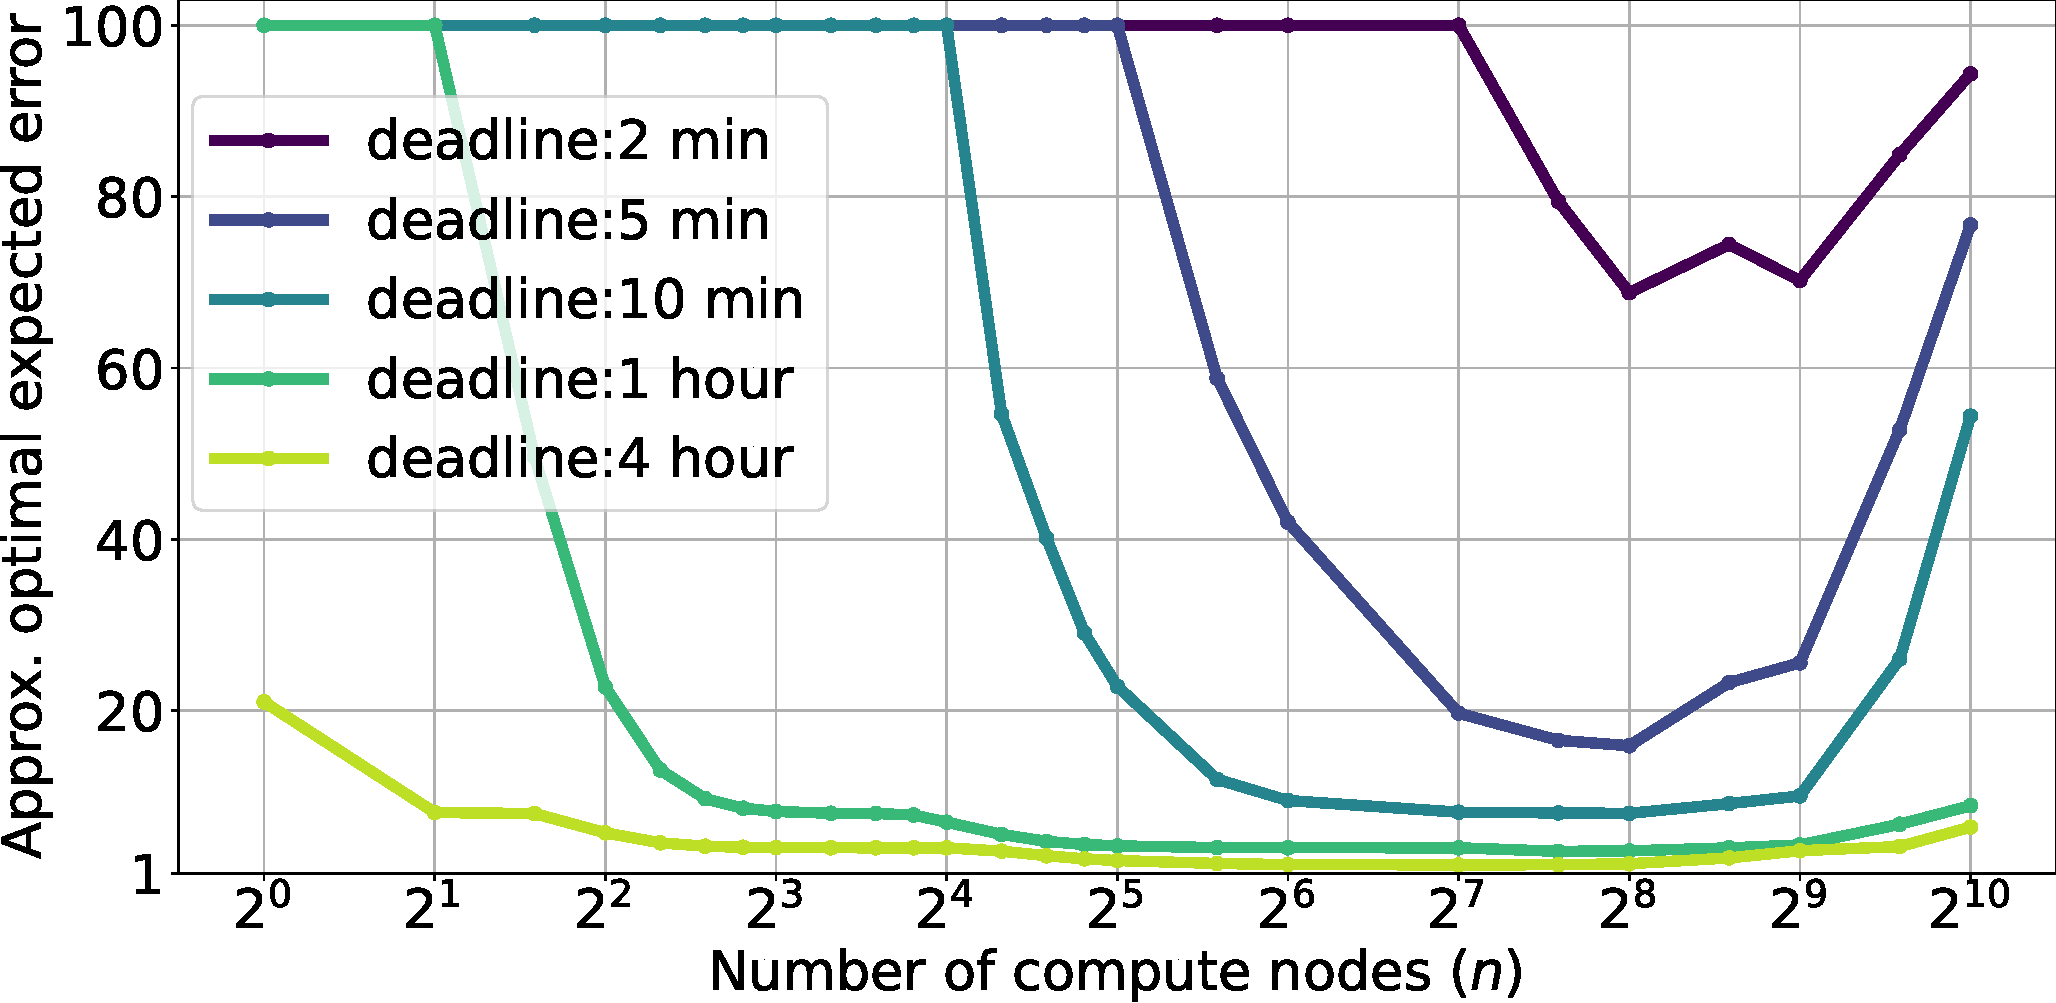
\includegraphics[width=\columnwidth]{./figures/data_parallel_results.pdf}	
	\caption{Approximate optimal expected error vs. number of compute nodes for different deadlines, for the fusion use case in Section~\ref{sec:use-case}.}
	\label{fig:data_parallel}
\end{figure}

Fig.~\ref{fig:data_parallel} shows the approximate optimal expected
error, as computed using the results in Section~\ref{sec:onehost:solution},
vs. $n$ for our fusion science use case.  Using a simple Amdahl parallel
speedup model, the fraction of the sequential execution that is
parallelizable is $0.89$, $0.99$, and $0.99$ for tasks $T_1$, $T_2$, and
$T_3$, respectively. These values are based on results
in~\cite{9912722} and on information provided to us by the authors.  As
seen in the figure, the tighter the deadline, the more compute nodes are
necessary to achieve an expected error below \efail (which is set to 100
in these experiments). For instance, doing so
for a 5-minute deadline requires $n{>}32$ compute nodes.  
But using as many compute nodes as possible is not advisable because the
failure rate increases with $n$.  There is thus a ``sweet spot" where
$n$ is large enough for parallelization to be useful but small enough that
failures are not too frequent.  Note that, for the shorter deadlines, the
curves appear more jagged. This is because
$\deltat{=}5$ is larger relative to the deadline, leading to a coarser 
discretization (using a smaller $\deltat$ value
would yield more precise approximations
of the optimal expected error for these shorter
deadlines). Overall, such results 
allow a user to make informed decisions, e.g., select a value of $n$ and a
deadline that achieve a desirable compromise between hardware cost,
timeliness, and expected error.

%\subsection{In-Situ Executions}
%
%Another application of our results is provide a sound comparison of different execution
%options. For instance, one may wish to determine whether on should execute
%that task chain in an ``in-situ" manner, i.e., keeping all task input/output data
%in memory. While this reduces application execution time by removing all I/O
%operations, but requires a re-execution from scratch when a failure occurs.
%
%\TODO{This section is perhaps unnecessary. We should update the code to allow in-situ executions. Done with the USE CASE}


\subsection{Evaluation of Simple Heuristics}
\label{sec:onehost:heuristics}

Our dynamic programming approach is usable in practice. It also
provides a reference against which heuristics can be compared and evaluated.
This is useful to determine which scheduling principles are effective in the 
one-PE case, and may be worth reusing in the multi-PE case.

We consider four criteria for selecting a task's execution mode:
(\errorlevel)~the lowest error level;
(\probsuccess)~the highest probability of success by the deadline; (\ratio)~the
highest ratio of probability of success to error level; and (\expectederror)~the
lowest expected error by the deadline. Criterion \expectederror criterion is computed using the recursion in Section~\ref{sec:onehost:solution}, while criteria \probsuccess and \ratio
are computed using modified versions of that recursion.  We then consider two categories of heuristics:
\begin{compactitem}	
	\item \textbf{Nearsighted} (\textsc{Ns}) - When selecting the execution mode for the next task using the chosen criterion, assume that this task is the last task in the chain. 
	\item \textbf{Foresighted} (\textsc{Fs}) - At the onset of the application execution, 
	analyze each possible combination of execution modes for all tasks and select 
	the combination that optimizes for the chosen criterion.
\end{compactitem}
\noindent
We denote each heuristic by its category and criterion, e.g., heuristic
\foresighted-\expectederror is the foresighted heuristic that uses the
lowest-expected-error criterion. All these heuristics are static, i.e.,
once an execution mode has been decided for a task, that same mode is used
for any re-executions of that task.  Finally, we consider a baseline
heuristic, \random, that picks task execution modes randomly,  for a total
of $4{\times}2{+}1{=}9$ heuristics.



We evaluate our dynamic programming approach, which we denote by \dynamic, along
with the above nine heuristics in simulation, for 500 different synthetic
application configurations and 20 random trials per configuration. We use
two different $\efail$ multipliers, i.e., $\efail$ is set to either 2$\times$ or
5$\times$ the highest possible error that a successful application execution can
achieve.  All findings and rankings hereafter are unchanged
when considering results for different multiplier values separately, and we
only discuss combined results.  The use of temporal redundancy can only be
beneficial, and our results show improvements in mean error ranging from 0\% to
8.97\% for all our heuristics, with an average improvement of 2.18\%. In
all that follows, we only discuss results with temporal redundancy enabled.

\begin{figure}[ht!]
	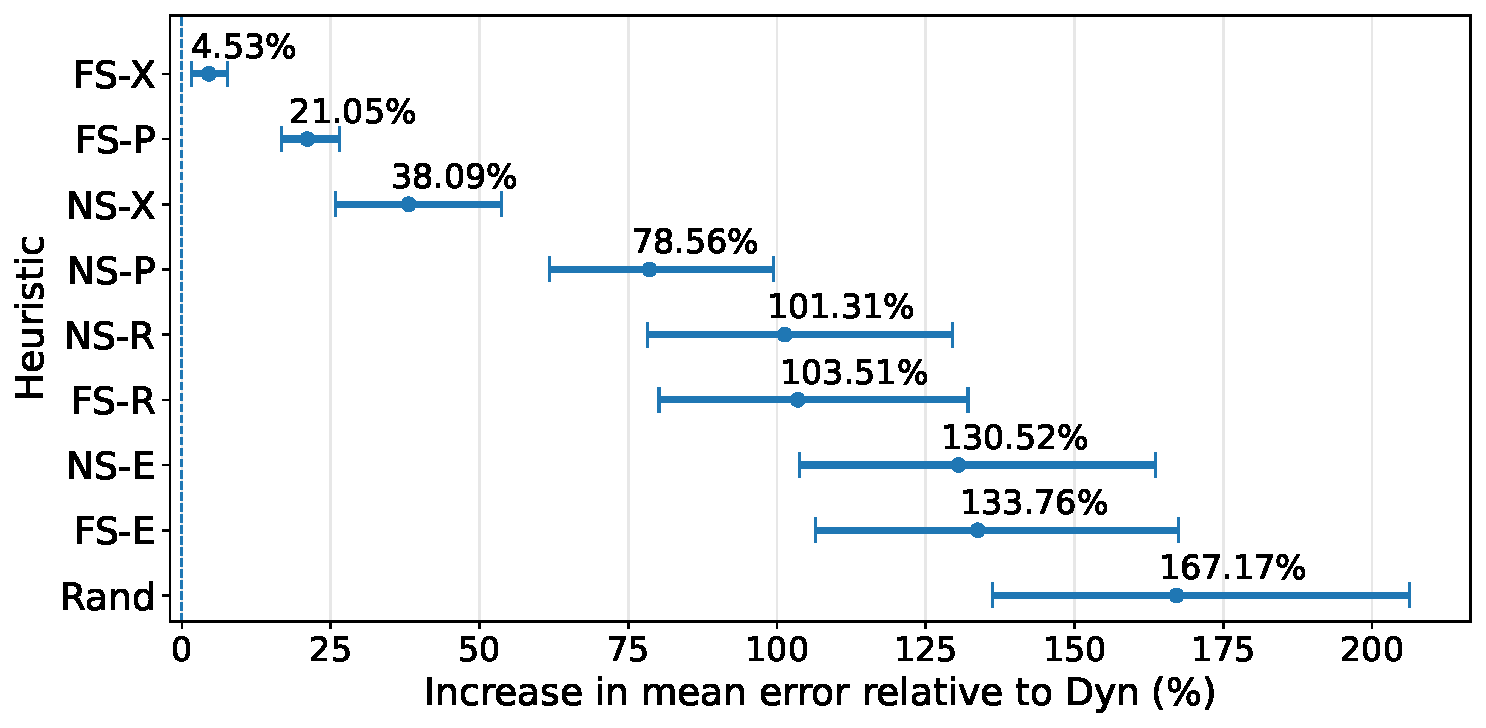
\includegraphics[width=\columnwidth]{./figures/relative_error_vs_dynamic.pdf}
	\caption{Mean error increases relative to the dynamic programming approach in the one-PE case (95\% paired-bootstrap confidence intervals shown).}
	\label{fig:one_host_results}
\end{figure}


We compare a heuristic $H$ to \dynamic using
the relative difference in expected error, $(\mu_H-\mu_{\dynamic})/\mu_\dynamic$,
where $\mu$ denotes the achieved expected error.  We
estimate this quantity using the corresponding sample means and compute a
95\% paired percentile-bootstrap confidence interval. 
Fig.~\ref{fig:one_host_results} shows these intervals
for all heuristics. \dynamic outperforms all heuristics, since no confidence interval contains the value zero. As expected, \random
performs the worst. We find that among the four criteria, the ranking from
best to worst is \expectederror (expected error), \probsuccess (probability of
success), \ratio (probability of success to error level ratio), and
\errorlevel (error level). This is also expected because criterion
\expectederror is the most directly related to the mean error objective, while
criterion \errorlevel, which comes last, is the least related. 
In terms of heuristic
categories, for the bottom two criteria (\ratio and \errorlevel), the
\nearsighted and \foresighted versions perform similarly, with a small
advantage to \nearsighted. However, for the top two criteria (\expectederror and \probsuccess), the
\foresighted heuristic outperforms the \nearsighted version.  This
intuitively makes sense: the quality of the criterion magnifies the
quality of longer-term planning.

Overall, the top-performing heuristic is \foresighted-\expectederror
(foresighted with the lowest expected error as the criterion), with a mean error increase
of 4.53\% relative to \dynamic. In our results, out of 20,000 experiments, 
\foresighted-\expectederror and \dynamic tie in 11,584 cases, \dynamic
wins in 7,106 cases and loses in 1,310 cases. 
\dynamic is not guaranteed
to produce the lowest error for every particular failure trace: it
minimizes expected error rather than the error for a particular realization
of the failure process. 
To ascertain the sensitivity of the above results to the
(number of) samples, we performed 500 random split-half analyses (keeping
all experiments associated with the same application configuration in the
same half). \dynamic ranked first and \foresighted-\expectederror ranked second
in 100\% of the half-samples.


